\documentclass[main-ap-physics.tex]{subfiles}


\begin{document}

\subsection{Vector Addition and Subtraction: Graphical Methods}

\subsubsection*{Vectors in Two Dimensions}

A \gls{vector} is a quantity that has magnitude and direction. Displacement, velocity, acceleration, and force, for example, are all vectors. In one-dimensional, or straight-line, motion, the direction of a vector can be given simply by a plus or minus sign. In two dimensions (2-d), however, we specify the direction of a vector relative to some reference frame (i.e., coordinate system), using an arrow having length proportional to the vector's magnitude and pointing in the direction of the vector.

\vspace{1em}
Figure ?.?? shows such a graphical representation of a vector, using as an example the total displacement for the person walking in a city considered in Kinematics in Two Dimensions: An Introduction. We shall use the notation that a boldface symbol, such as $\mathbf{D}$, stands for a vector. Its magnitude is represented by the symbol in italics, \textbf{\textit{D}}, and its direction by $\theta$.

\begin{gradient}{VECTORS IN THIS TEXT}
    In this text, we will represent a vector with a boldface variable. For example, we will represent the quantity force with the vector $\textbf{F}$, which has both magnitude and direction. The magnitude of the vector will be represented by a variable in italics, such as \textbf{\textit{F}}, and the direction of the variable will be given by an angle $\theta$.
\end{gradient}

\begin{center}
    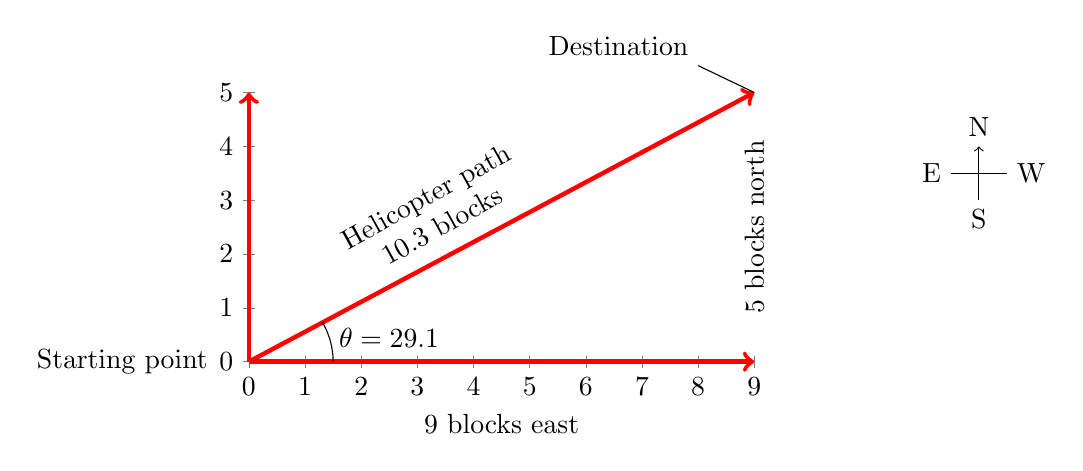
\begin{tikzpicture}
        \begin{axis}[width=8cm, height=5cm,
            xmin=0,xmax=9,
            ymin=0,ymax=5,
            xtick={0,1,...,9},
            ytick={0,1,...,5},
            clip=false,
            axis lines = left,
            xlabel={9 blocks east},
        ]
        \draw[->,ultra thick,red] (0,0) -- (9,0);
        \draw[->,ultra thick,red] (0,0) -- ++(0,5);
        \draw[->,ultra thick,red] (0,0) -- (9,5) node[pos=0.6, above left=1mm,rotate=29,align=center,black] {Helicopter path\\10.3 blocks} node[black,below,pos=0.5,rotate=29] {\Large \myheli};
        \node[left=4mm] at (0,0) {Starting point};
        \draw (9,5) -- ++(-1,0.5) node[above left] {Destination};
        \draw (1.5,0) arc (0:29.1:1.5) node[right,pos=0.6] {$\theta = \ang{29.1}$};
        \node[rotate=90] at (9,2.5) {5 blocks north};
        \begin{scope}[shift={(13,3)}]
            \draw[->] (0,0) node[below] {S} -- ++(0,1) node[above] {N};
            \draw (-0.5,0.5) node[left] {E} -- ++(1,0) node [right] {W};
        \end{scope}
        \end{axis}
    \end{tikzpicture}
    \captionsetup{type=figure,margin=1in,font=scriptsize}
    \captionof{figure}{A person walks 9 blocks east and 5 blocks north. The displacement is 10.3 blocks at an angle \ang{29.1} north of east.}
\end{center}

\begin{center}
    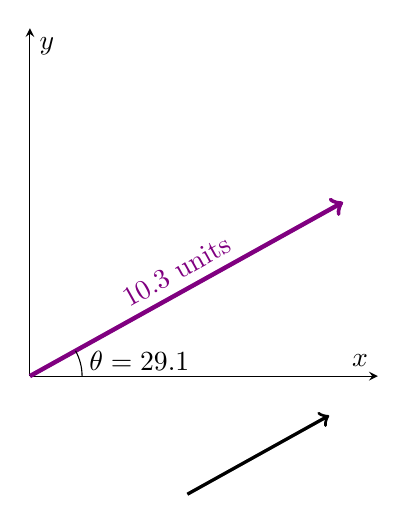
\begin{tikzpicture}
        \begin{axis}[width=6cm,height=6cm,
            xmin=0,xmax=10,
            ymin=0,ymax=10,
            ticks=none,
            axis lines=center,
            xlabel={$x$},
            ylabel={$y$},
            clip=false
        ]
        \draw[ultra thick,violet,->] (0,0) -- ++(9,5) node[pos=0.5,above,rotate=29.1] {10.3 units};
        \draw (1.5,0) arc (0:29:1.5) node[pos=0.6,right] {$\theta = \ang{29.1}$};
        \end{axis}
        \tkzRegle[Fond=true,Opacite=0.9,CouleurFond=yellow,AfficheValeurs=false,Origine={(-0.5,1)},Echelle=0.4,Rotation=29.1]
        \tkzRapporteur[Fond,CouleurFond=blue,Echelle=0.3,Origine={(2,-1.5)},AfficheAngles=false]
        \draw[very thick,->] (2,-1.5) -- ++(0.2*9,0.2*5);
    \end{tikzpicture}
    \captionsetup{type=figure,margin=1in,font=scriptsize}
    \captionof{figure}{To describe the resultant vector for the person walking in a city considered in Figure ?.?? graphically, draw an arrow to represent the total displacement vector $\textbf{D}$. Using a protractor, draw a line at an angle $\theta$ relative to the east-west axis. The length \textbf{\textit{D}} of the arrow is proportional to the vector's magnitude and is measured along the line with a ruler. In this example, the magnitude \textbf{\textit{D}} of the vector is 10.3 units, and the direction $\theta$ is \ang{29.1} north of east.}
\end{center}

\subsubsection*{Vector Addition: Head-to-Tail Method}

The head-to-tail method is a graphical way to add vectors, described in Figure ?.?? below and in the steps following. The tail of the vector is the starting point of the vector, and the head (or tip) of a vector is the final, pointed end of the arrow.

\begin{center}
    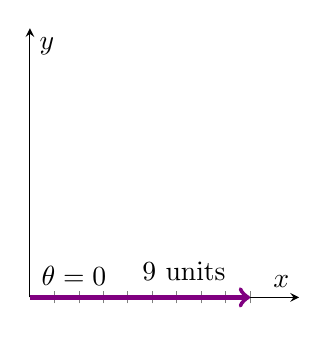
\begin{tikzpicture}
        \begin{axis}[width=5cm,height=5cm,
            xmin=0,xmax=11,
            ymin=0,ymax=11,
            axis lines=center,
            xlabel={$x$},
            ylabel={$y$},
            clip=false,
            xtick={0,1,...,9},
            ytick=\empty,
            xticklabels={},
        ]
        \draw[ultra thick,violet,->] (0,0) -- ++(9,0) node[pos=0.2,above,black] {$\theta = \ang{0}$} node[pos=0.7,above=2pt,black] {9 units};
        \end{axis}
    \end{tikzpicture}%
    \hspace{1em}
        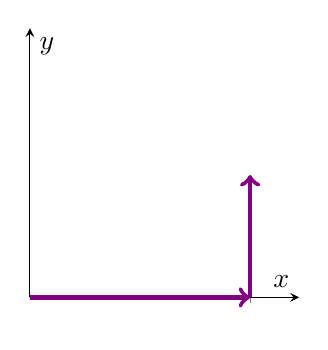
\begin{tikzpicture}
        \begin{axis}[width=5cm,height=5cm,
            xmin=0,xmax=11,
            ymin=0,ymax=11,
            axis lines=center,
            xlabel={$x$},
            ylabel={$y$},
            clip=false,
            xtick={9},
            ytick=\empty,
            xticklabels={},
        ]
        \draw[ultra thick,violet,->] (0,0) -- ++(9,0);
        \draw[ultra thick,violet,->] (9,0) -- ++(0,5);
        \end{axis}
    \end{tikzpicture}
    \captionsetup{type=figure,margin=1in,font=scriptsize}
    \captionof{figure}{}
\end{center}
\end{document}



